\subsection{Language coverage}

The first statistics consists of determining how much of the language is covered by the k most used words. The result is shown in figure \ref{coverage_figure}. We could see that, with the same amount of words, we cover less and less of the language from 1840 to 1995.

\begin{figure}[H]
	\centering
    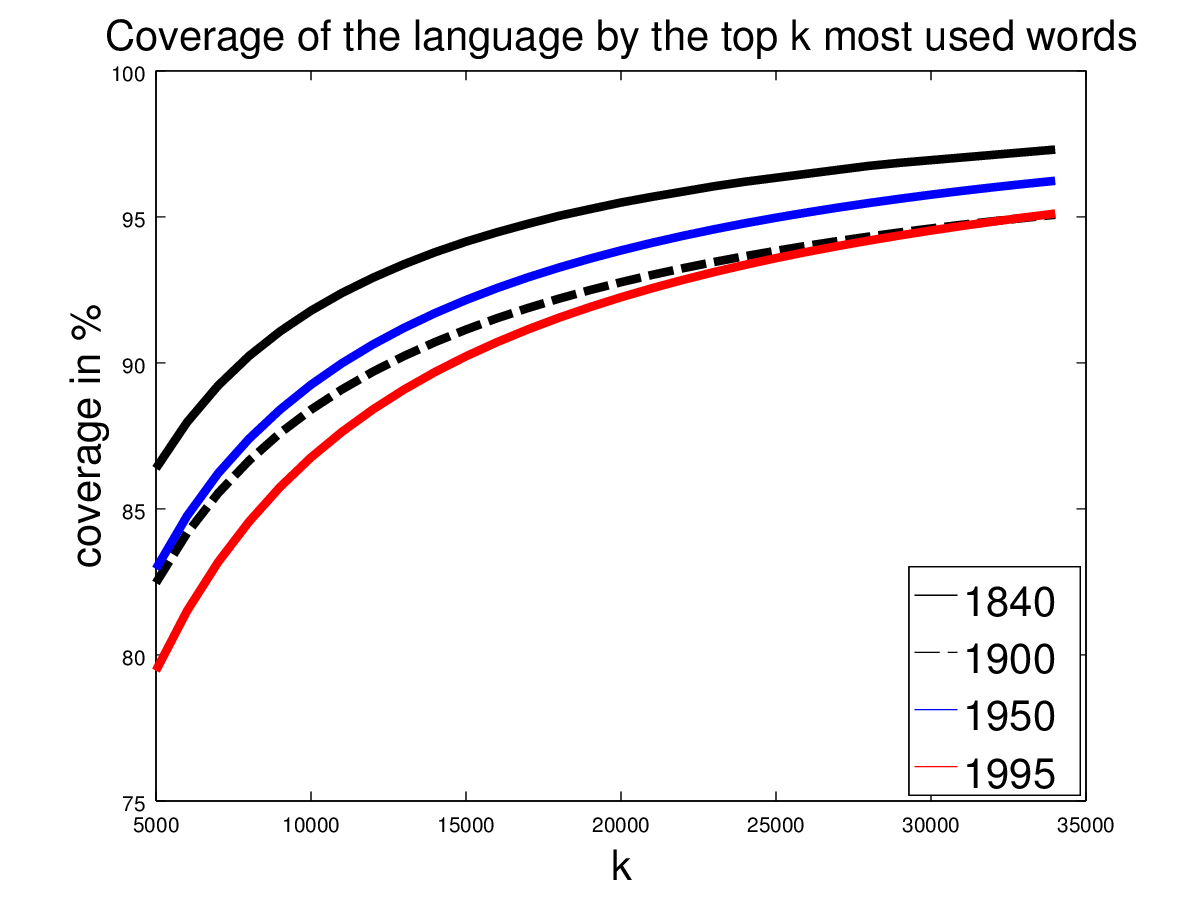
\includegraphics[scale=0.50]{Pictures/statistics/top-k-words-coverage/coverage.png}
    \caption{Percentage of text covered by the top k most used words}
    \label{coverage_figure}
\end{figure}

Those results can be interpreted in multiple ways. One way is to conclude that the appearance of words is faster than disappearance. But, this could also show that there are more and more variations in our vocabulary.